\documentclass{standalone}
\usepackage{tikz}
\usetikzlibrary{automata, positioning}

\begin{document}
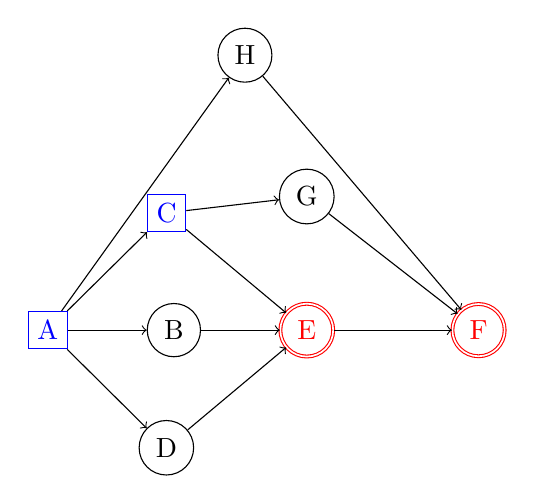
\begin{tikzpicture}[normal/.style = {draw, circle}, dfork/.style = {draw, rectangle, blue}, djoin/.style = {draw, double, circle, red}]
  \node[dfork] (a) at (1,1) {A};
  \node[normal, right = of a] (b) {B}; 
  \node[dfork, above right = of a] (c) {C}; 
  \node[normal, below right = of a] (d) {D}; 

  \node[djoin, right = of b] (e) {E}; 
  \node[djoin, right = 1.5cm of e] (f) {F}; 

  \node[normal, above = of e] (g) {G}; 
  \node[normal, above right = 3.0cm and 2.0cm of a] (h) {H}; 

  \path (a) edge[->] (b)
	(a) edge[->] (c)
	(a) edge[->] (d)
	(a) edge[->] (h)
  	(b) edge[->] (e) 
	(c) edge[->] (e)
	(c) edge[->] (g)
	(d) edge[->] (e)
	(e) edge[->] (f)
	(g) edge[->] (f)
	(h) edge[->] (f); 
\end{tikzpicture}
\end{document}